%
% explizit.tex
%
% (c) 2020 Prof Dr Andreas Müller, Hochschule Rapperswil
%
\begin{frame}
\frametitle{Explizite Verfahren}
\vspace{-15pt}
\begin{columns}[t]
\begin{column}{0.48\hsize}
\begin{block}{Wärmeleitungsgleichung}
\vspace{-15pt}
\begin{align*}
\frac{\partial u}{\partial t}
&=
\frac{\partial^2 u}{\partial x^2}
&&\text{in $\mathbb R\times\mathbb R^+$}
\\
u(x,0)&=g(x)&&\text{auf $\mathbb R\times \{0\}$}
\end{align*}
\end{block}
\vspace{-10pt}
\uncover<3->{%
\begin{block}{Euler-Verfahren}
\vspace{-15pt}
\begin{align*}
\frac{u_{i,j+1}-u_{i,j}}{\Delta t}
&= 
\frac{u_{i+1,j}-2u_{i,j}+u_{i-1,j}}{\Delta x^2}
=
\frac{1}{\Delta x^2}(Lu)_{ij}
\\
u_{i,j+1}
&=
u_{i,j} + \Delta t
\frac{u_{i+1,j}-2u_{i,j}+u_{i-1,j}}{\Delta x^2}
\end{align*}
\end{block}}
\vspace{-15pt}
\uncover<4->{%
\begin{block}{Vektorschreibweise}
$u_j=\mathstrut$ Zeile $j$ von $u_{ij}$, $A = \frac{\Delta t}{\Delta x^2}L$
\begin{align*}
u_{j+1} &=  u_j + Au_j = (A+E)u_j
\end{align*}
\end{block}}
\end{column}
\begin{column}{0.48\hsize}
\uncover<2->{%
\begin{block}{Diskretisation}
\vspace{-15pt}
\begin{align*}
\frac{\partial u}{\partial t}
&=
\frac{u_{i,j+1}-u_{ij}}{\Delta t}
\\
\frac{\partial^2u}{\partial x^2}
&=
\frac{u_{i+1,j}-2u_{i,j}+u_{i-1,j}}{\Delta x^2}
\end{align*}
\begin{center}
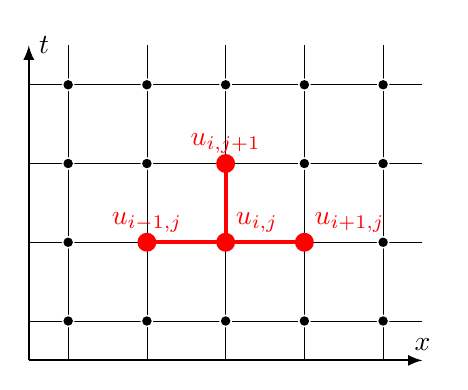
\begin{tikzpicture}[>=latex,thick]
\foreach \x in {-2,...,2}{
	\draw[line width=0.2pt] (\x,-1.5)--(\x,2.5);
}
\foreach \y in {-1,...,2}{
	\draw[line width=0.2pt] (-2.5,\y)--(2.5,\y);
}
\foreach \x in {-2,...,2}{
	\foreach \y in {-1,...,2}{
		\fill[color=white] (\x,\y) circle[radius=0.08];
		\fill (\x,\y) circle[radius=0.06];
	}
}
\fill[color=red] (-1,0) circle[radius=0.12];
\fill[color=red] (0,0) circle[radius=0.12];
\fill[color=red] (1,0) circle[radius=0.12];
\fill[color=red] (0,1) circle[radius=0.12];
\draw[color=red,line width=1.5pt] (-1,0)--(1,0);
\draw[color=red,line width=1.5pt] (0,0)--(0,1);

\node[color=red] at (0,0) [above right] {$u_{i,j}\mathstrut$};
\node[color=red] at (1,0) [above right] {$u_{i+1,j}\mathstrut$};
\node[color=red] at (-1,0) [above] {$u_{i-1,j}\mathstrut$};
\node[color=red] at (0,1) [above] {$u_{i,j+1}\mathstrut$};

\draw[->] (-2.5,-1.5) -- (2.5,-1.5) coordinate[label={$x$}];
\draw[->] (-2.5,-1.5) -- (-2.5,2.5) coordinate[label={right:$t$}];

\end{tikzpicture}
\end{center}
\end{block}}
\end{column}
\end{columns}

\end{frame}
